\chapter{Histogram Equalization}

\section{Problem statement}

\begin{enumerate}
    \item Write a computer program for computing the histogram of an image.\\
    \item Implement the histogram equalization technique.\\
    \item Your program must be general to allow any gray-level image as its input.\\
\end{enumerate}

\section{Python implementation}

Usage:~\textbf{python problem1.py [-h] image\_path}

\section{Figure 1}

    \subsection{Histogram}

    Original image:~\ref{diagram:fig1} |
    Original image's histogram:~\ref{diagram:hist_fig1}

    \begin{figure}[!htb]\centering
        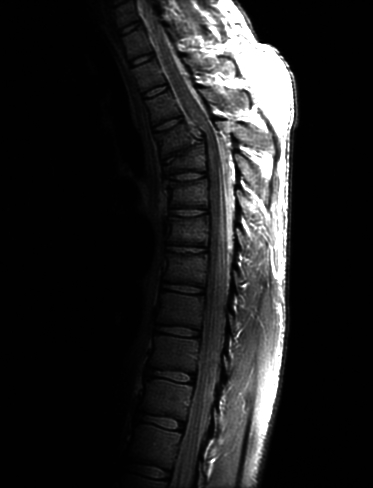
\includegraphics[width=0.7\linewidth]{./images/1/Fig1.jpg}
        \caption{Original \textit{Fig1.jpg}}\label{diagram:fig1}
    \end{figure}

    \begin{figure}[!htb]\centering
        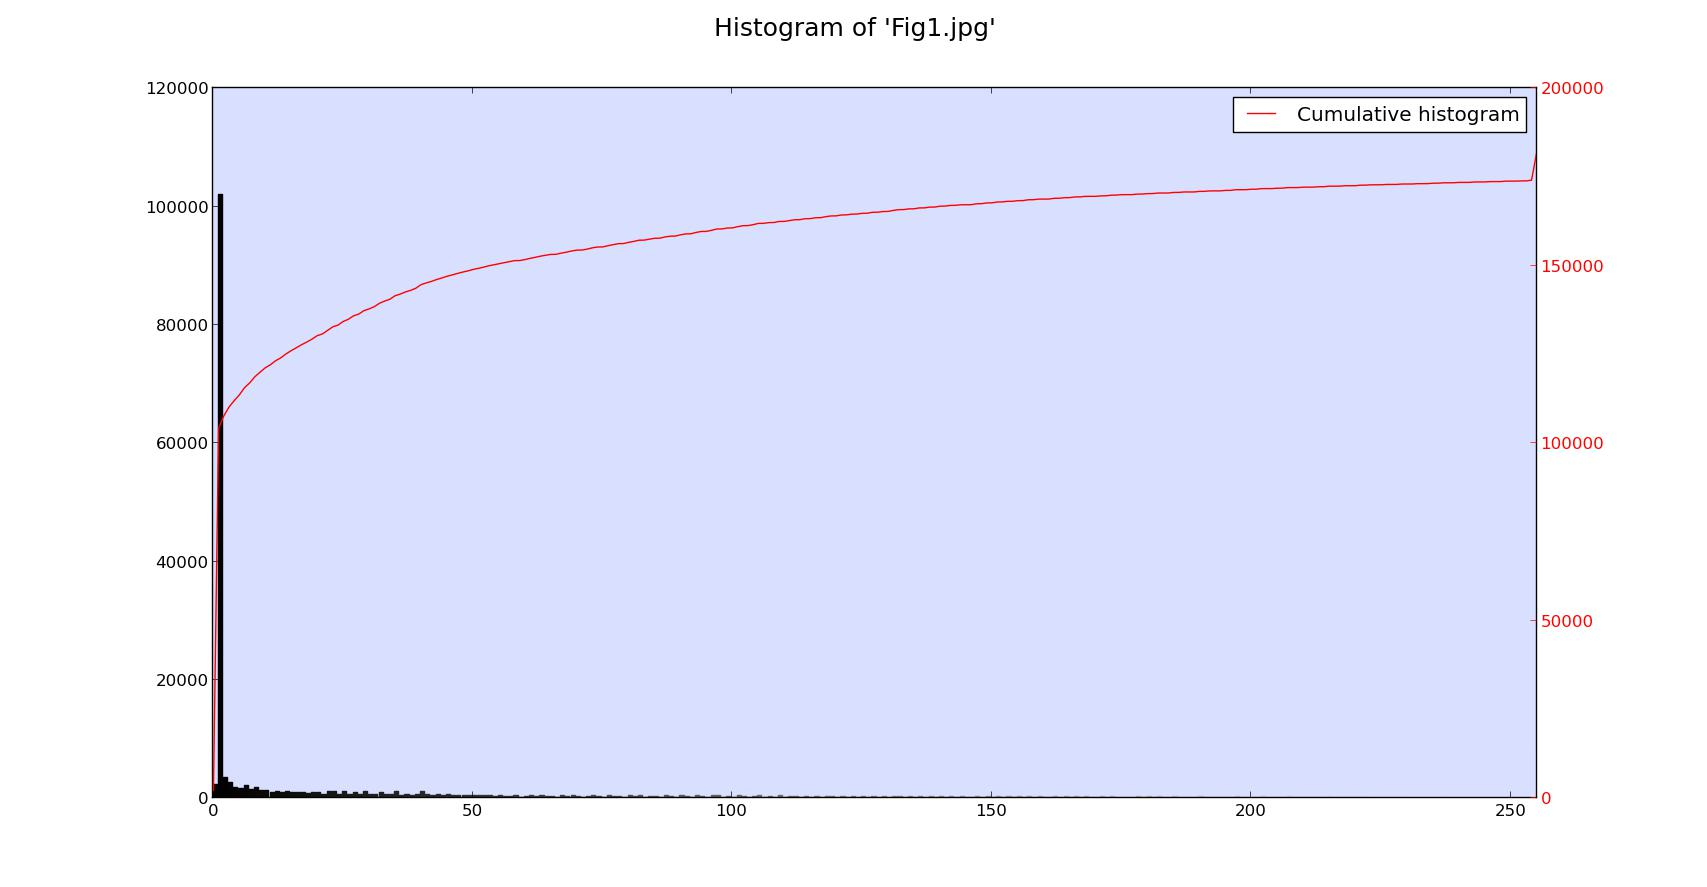
\includegraphics[width=\linewidth]{./images/1/Histogram_Fig1.jpg}
        \caption{Histogram of \textit{Fig1.jpg}}\label{diagram:hist_fig1}
    \end{figure}

    \subsection{Histogram equalization}

    Enhanced image:~\ref{diagram:enhanced_fig1} |
    Enhanced image's histogram:~\ref{diagram:equal_hist_fig1}

    \begin{figure}[!htb]\centering
        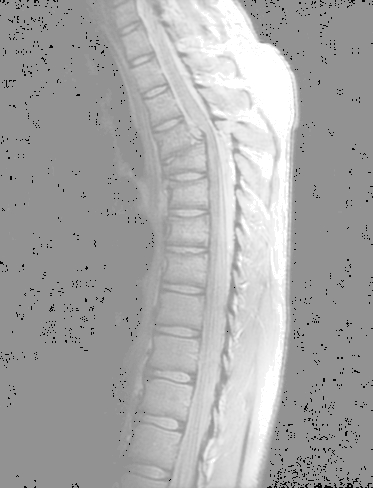
\includegraphics[width=0.7\linewidth]{./images/1/Enhanced_Fig1.jpg}
        \caption{Enhanced \textit{Fig1.jpg}}\label{diagram:enhanced_fig1}
    \end{figure}

    \begin{figure}[!htb]\centering
        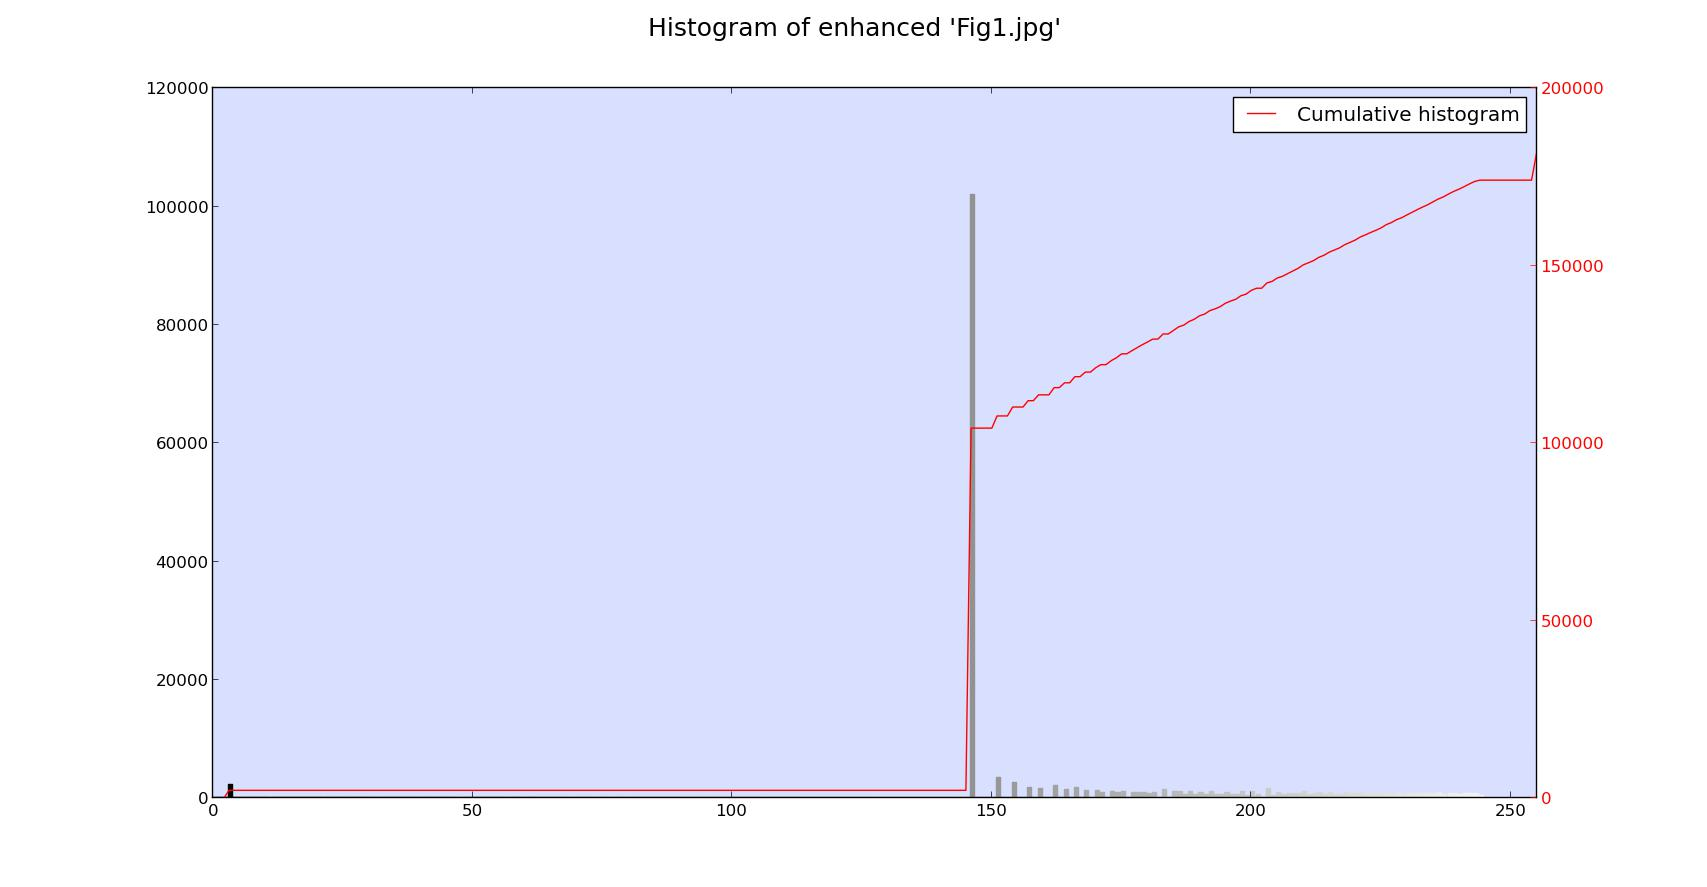
\includegraphics[width=\linewidth]{./images/1/Equalized_Histogram_Fig1.jpg}
        \caption{Equalized histogram of \textit{Fig1.jpg}}\label{diagram:equal_hist_fig1}
    \end{figure}


\section{Figure 2}

    \subsection{Histogram}

    Original image:~\ref{diagram:fig2} |
    Original image's histogram:~\ref{diagram:hist_fig2}

    \begin{figure}[!htb]\centering
        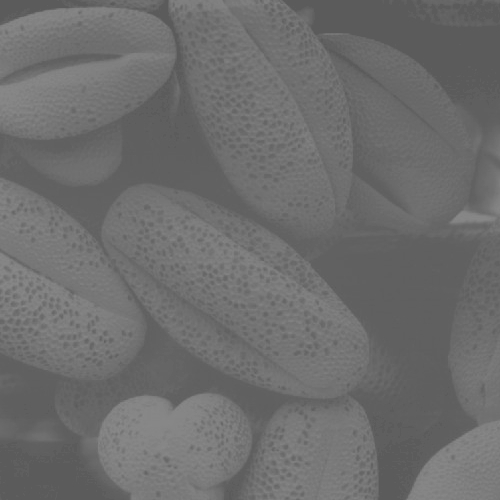
\includegraphics[width=0.7\linewidth]{./images/1/Fig2.jpg}
        \caption{Original \textit{Fig2.jpg}}\label{diagram:fig2}
    \end{figure}

    \begin{figure}[!htb]\centering
        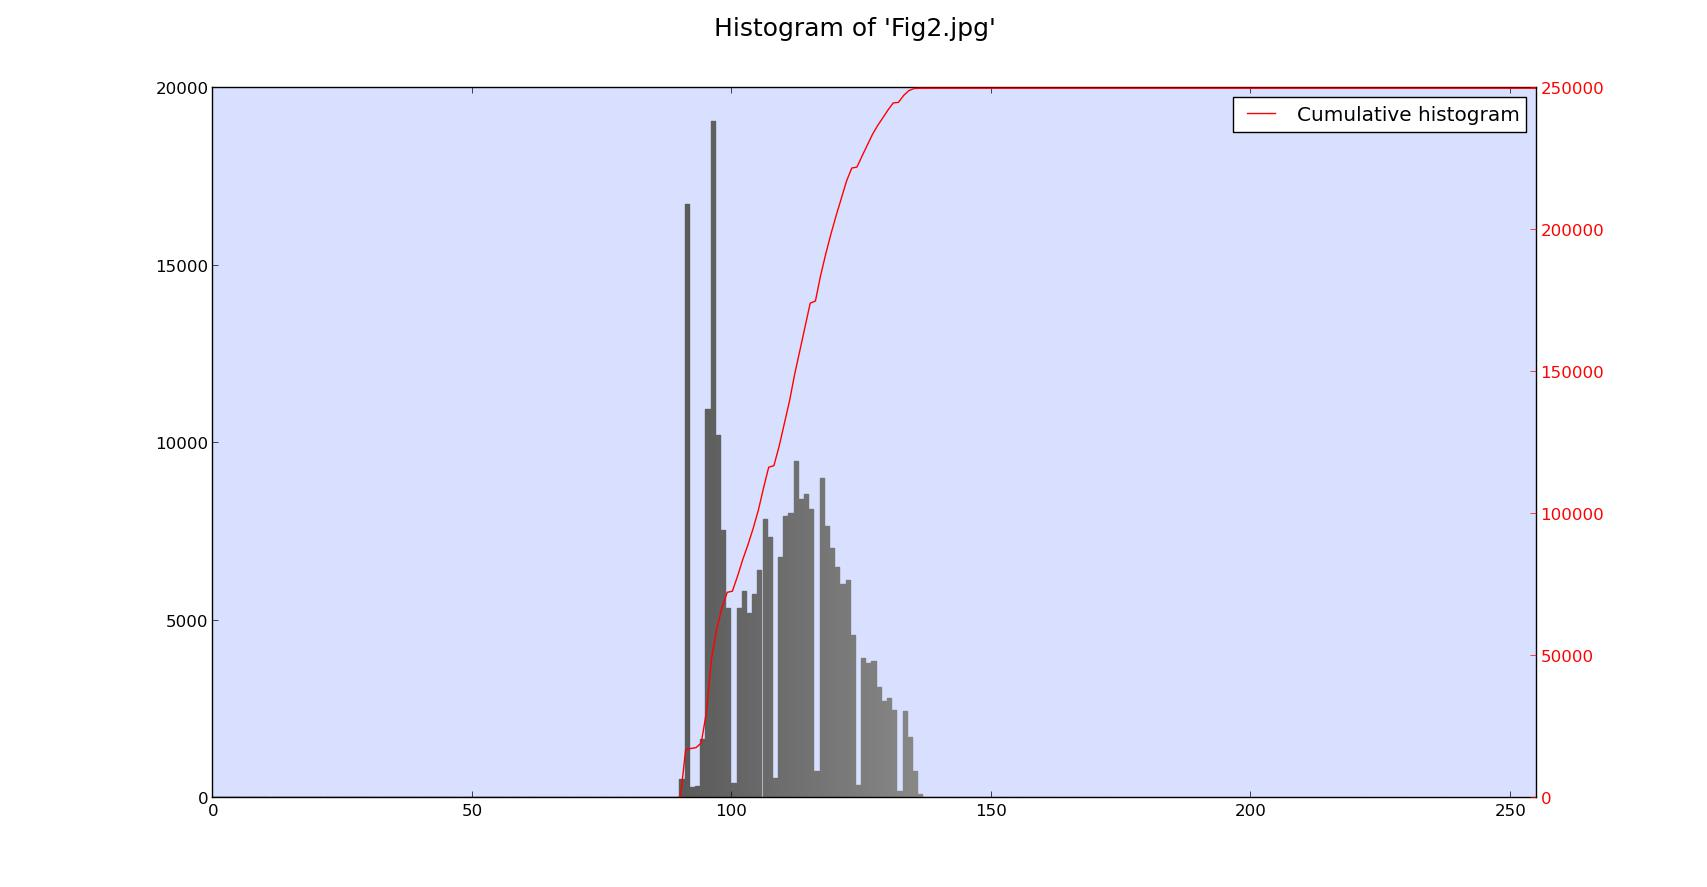
\includegraphics[width=\linewidth]{./images/1/Histogram_Fig2.jpg}
        \caption{Histogram of \textit{Fig2.jpg}}\label{diagram:hist_fig2}
    \end{figure}

    \subsection{Histogram equalization}

    Enhanced image:~\ref{diagram:enhanced_fig2} |
    Enhanced image's histogram:~\ref{diagram:equal_hist_fig2}

    \begin{figure}[!htb]\centering
        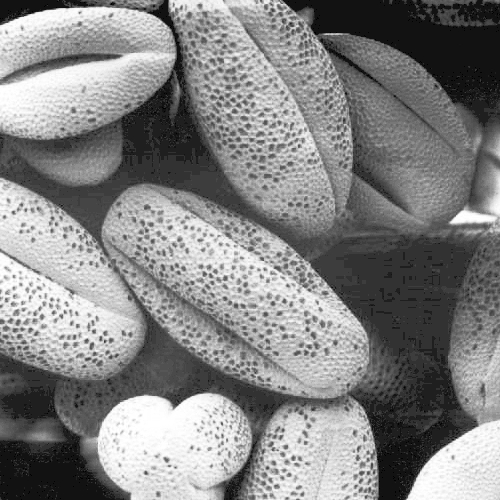
\includegraphics[width=0.7\linewidth]{./images/1/Enhanced_Fig2.jpg}
        \caption{Enhanced \textit{Fig2.jpg}}\label{diagram:enhanced_fig2}
    \end{figure}

    \begin{figure}[!htb]\centering
        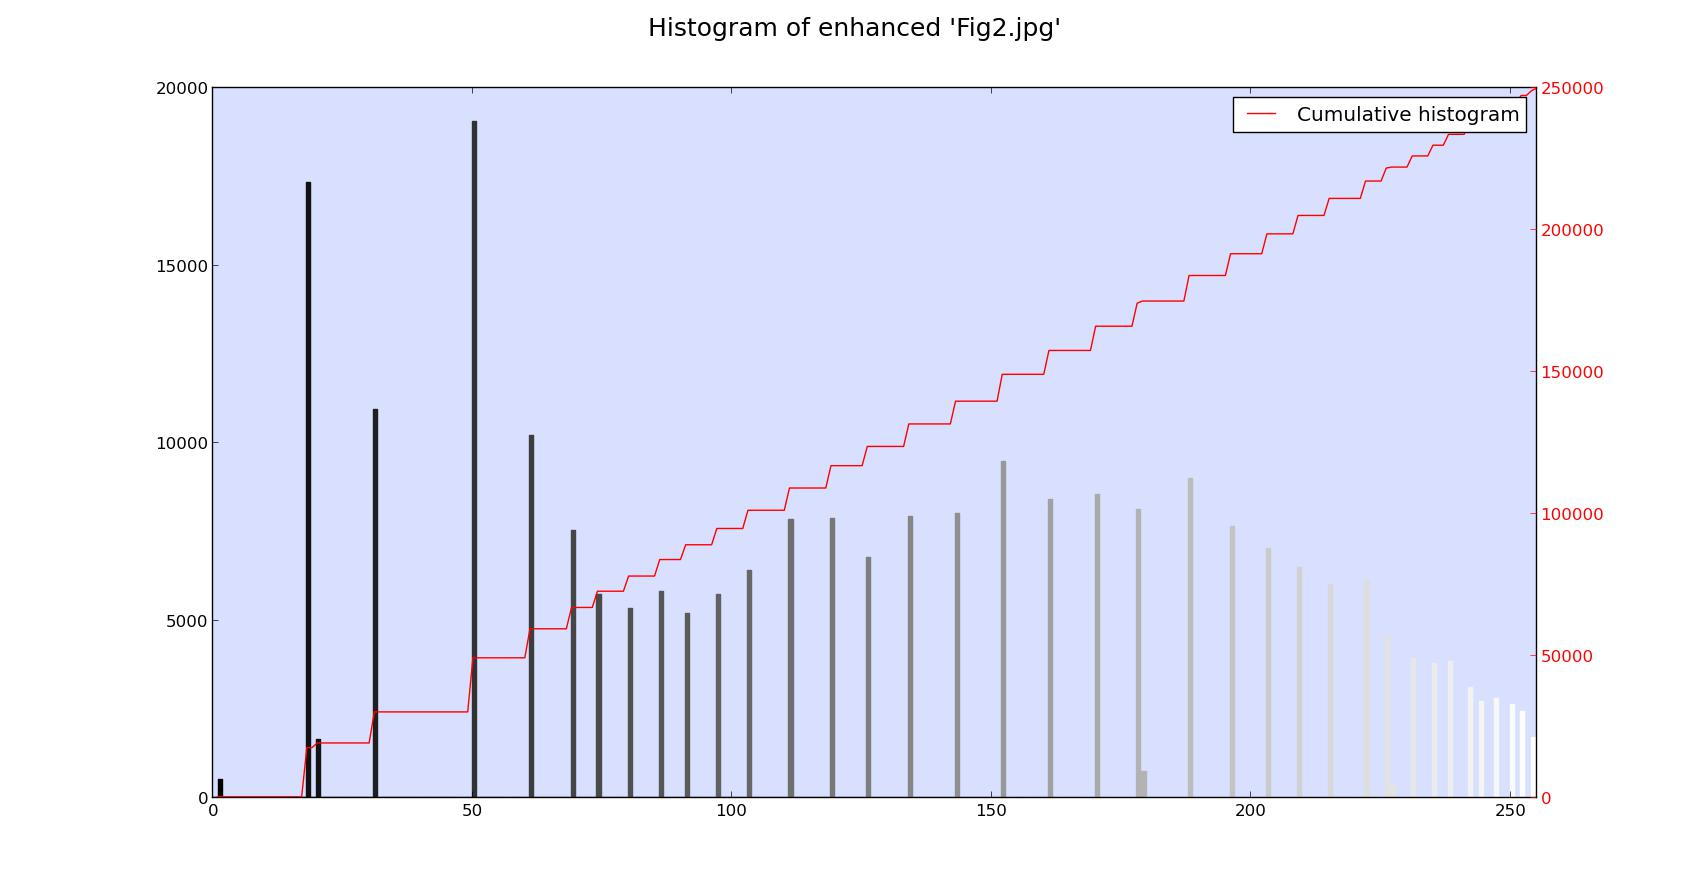
\includegraphics[width=\linewidth]{./images/1/Equalized_Histogram_Fig2.jpg}
        \caption{Equalized histogram of \textit{Fig2.jpg}}\label{diagram:equal_hist_fig2}
    \end{figure}
